\label{ndbt}

\tikzset{blue}

%\subsection{Dans un n\oe ud de Tikz}
\SbSSCT{Dans un n\oe ud de Tikz}{In a TikZ node}
\label{noeudboite}

\begin{tabular}{|c | c | c | c |} \hline
\multicolumn{4}{|c|}{ \BS{tikz} \BS{draw} (0,0) grid (2,2) (1,1) node[fill=red!20,] \AC{texte};   }\\ 
\hline 
\tikz \draw (0,0) grid (2,2) (1,1) node[fill=red!20] {texte};
&
\tikz \draw (0,0) grid (2,2) (1,1) node[fill=red!20,draw] {texte}; 
&
\tikz \draw (0,0) grid (2,2) (1,1) node[circle,fill=red!20] {texte};
&
\tikz \draw (0,0) grid (2,2) (1,1) node[circle,fill=red!20,draw] {texte};
\\  \hline
node[fill=red!20] 
&
node[fill=red!20,\RDD{draw}] 
&
 node[fill=red!20,\RDD{circle}]  
&
 node[fill=red!20,\RDD{circle},\RDD{draw}]
 \\  \hline
\end{tabular}
\bigskip


\subsubsection{Options}
\begin{tabular}{|c | c | c | c |c |c |c |c |} \hline
\multicolumn{8}{|c|}{ \BS{tikz} \BS{draw} node[draw,\RDD{double},blue] \AC{texte};   }\\ 
\hline 

\tikz \draw  node[draw,double,blue] {texte};
&
\tikz \draw  node[draw,rounded corners,blue] {texte};
&
\tikz \draw  node[draw,ultra thick,blue] {texte};
&
\tikz \draw  node[draw,dashed,blue] {texte};
&
\tikz \draw  node[draw,red] {texte};
&
\tikz \draw  node[draw,rotate=45,blue] {texte};
&
\tikz \draw  node[draw,shading=radial,blue] {texte};
&
\tikz \draw  node[draw,blue,text=red] {texte};
\\ \hline
\RDD{double} & \RDD{rounded corners} &  ultra thick & dashed & red & rotate=45 & shading=radial & text=red 
\\ \hline
\end{tabular}
\bigskip


\begin{tabular}{|c | c | c | c |c |} \hline
\multicolumn{4}{|c|}{ \BS{tikz} \BS{draw}  node[draw,\RDD{inner sep}=0pt] \AC{texte};   }\\ 
\hline 
\tikz \draw  node[draw,inner sep=0pt,blue] {texte};
&
\tikz \draw node[draw,inner sep=1cm,blue] {texte};
&
\tikz \draw  node[draw,inner xsep=1cm,blue] {texte};
&
\tikz \draw  node[draw,inner ysep=1cm,blue] {texte};
\\ \hline
 \RDD{inner sep}=0pt & \RDD{inner sep}=1cm & \RDD{inner xsep}=1cm & \RDD{inner ysep}=1cm
\\ \hline
\multicolumn{4}{|c|}{ \dft{} : 0.3333em }\\ 
\hline 

\end{tabular}

\bigskip

\begin{tabular}{|c | c | c | c |} \hline
\multicolumn{4}{|l|}{ \BS{node} [fill=red!20,\RDD{outer sep}=1cm] (A) at (1,1) \AC{texte};   }\\ 
\multicolumn{4}{|l|}{ \BS{fill} (node cs:name=A,anchor=east) circle (3pt);  }\\ 
\multicolumn{4}{|l|}{ \BS{fill} (node cs:name=A,anchor=south) circle (3pt);  }\\ 
\hline 
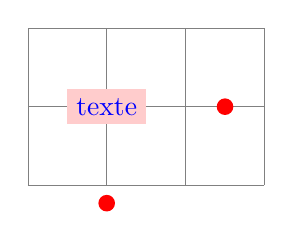
\begin{tikzpicture}
\draw[help lines] (0,0) grid (3,2);
\node[fill=red!20,outer sep=1cm] (A) at (1,1) {texte};
\fill[red] (node cs:name=A,anchor=east) circle (3pt);
\fill[red] (node cs:name=A,anchor=south) circle (3pt);
\end{tikzpicture}
&
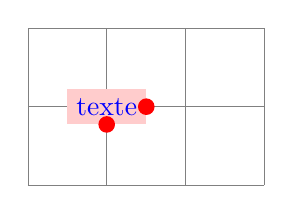
\begin{tikzpicture}
\draw[help lines] (0,0) grid (3,2);
\node[fill=red!20,outer sep=0pt] (A) at (1,1) {texte};
\fill[red] (node cs:name=A,anchor=east) circle (3pt);
\fill[red] (node cs:name=A,anchor=south) circle (3pt);
\end{tikzpicture}
&
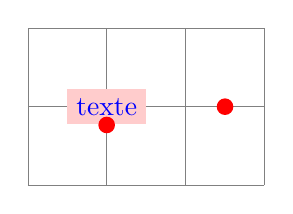
\begin{tikzpicture}
\draw[help lines] (0,0) grid (3,2);
\node[fill=red!20,outer xsep=1cm] (A) at (1,1){texte};
\fill[red] (node cs:name=A,anchor=east) circle (3pt);
\fill[red] (node cs:name=A,anchor=south) circle (3pt);
\end{tikzpicture}
&
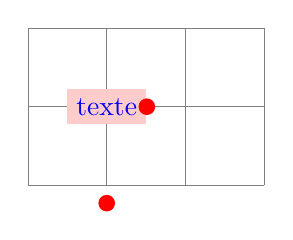
\begin{tikzpicture}
\draw[help lines] (0,0) grid (3,2);
\node[fill=red!20,outer ysep=1cm] (A) at (1,1) {texte};
\fill[red] (node cs:name=A,anchor=east) circle (3pt);
\fill[red] (node cs:name=A,anchor=south) circle (3pt);
\end{tikzpicture}
\\ \hline
 \RDD{outer sep}=1cm & \RDD{outer sep}=0pt & \RDD{outer xsep}=1cm & \RDD{outer ysep}=1cm
\\ \hline
\multicolumn{4}{|c|}{ \dft{} : 0.5\BS{pgflinewidth} }\\ 
\hline 
\end{tabular}
%----------------------------------------------------------------------------------
%\subsubsection{Taille minimale des noeuds}
\SbSbSSCT{Taille minimale des noeuds}{Minimum size}

\begin{tabular}{|c|c|} \hline  
\multicolumn{2}{|c|}{  \BS{draw}((0,0) node[fill=blue!20,\RDD{minimum height}=1.5cm,draw]  \AC{texte} ;   }\\ 
\hline 
\tikz \draw (0,0) node[fill=red!20,minimum height=1.5cm,draw] {texte};
&  
\tikz \draw (0,0) node[fill=red!20,minimum width=3cm,draw] {texte};

\\ \hline  

\RDD{minimum height}=1.5cm
&  
\RDD{minimum width}=3cm
\\ \hline  
\tikz \draw (0,0) node[fill=red!20,minimum size=1.5cm,draw] {texte};
&  
\tikz \draw (0,0) node[fill=red!20,minimum size=1.5cm,draw,circle] {texte};

\\ \hline 
\RDD{minimum size}=1.5cm,draw
&  
\RDD{minimum size}=1.5cm,circle

\\ \hline 
\end{tabular} 

\newpage
%-----------------------------------------------
%\subsection{Dans un n\oe ud à formes géométriques}
\SbSSCT{Dans un n\oe ud à formes géométriques}{Geometric Shapes nodes}

\label{lib-geom}
\label{formes}
%Insérer dans le préambule :

 \maboite{\BS{usetikzlibrary}\AC{shapes.geometric}}
 
 
\begin{center}
\RRR{67-3}
\end{center}
%\subsubsection{Formes disponibles}
\SbSbSSCT{Formes disponibles}{Available shapes}

\label{nd1}

\begin{tabular}{|c|c|c|c|} \hline  
\multicolumn{4}{|l|}{ 2 syntaxes :   }\\ 
\multicolumn{4}{|l|}{ \BS{tikz} \BS{node}[fill=green!20,\RDD{shape}=diamond,draw,blue] \AC{texte};   }\\ 
\multicolumn{4}{|l|}{ \BS{tikz} \BS{node}[fill=green!20,\RDD{diamond},draw] \AC{texte};   }\\ 
\hline 
\tikz  \node[fill=green!20,diamond,draw] {texte}; 
&  
\tikz  \node[fill=green!20,ellipse,draw] {texte};
&  
\tikz  \node[fill=green!20,trapezium, regular polygon sides=6,draw] {texte};
&
\tikz  \node[fill=green!20,semicircle,draw] {texte}; 
\\ \hline 
diamond & ellipse  & trapezium & semicircle
\\ \hline 
\tikz  \node[fill=green!20,star,draw] {texte};
&  
\tikz  \node[fill=green!20,regular polygon,draw] {texte};
&  
\tikz  \node[fill=green!20,isosceles triangle,draw] {texte};
&
\tikz  \node[fill=green!20,kite,draw] {texte};
\\ \hline 
star & regular polygon  & isosceles triangle & kite 
\\ \hline 
\tikz  \node[fill=green!20,dart,draw] {texte};
&
\tikz  \node[fill=green!20,circular sector,draw] {texte};
&
\tikz  \node[fill=green!20,cylinder,draw] {texte};
&

\\ \hline 
dart & circular sector & cylinder &
\\ \hline 
\end{tabular} 

%---------------------------------------------------------------------------------------
\subsubsection{Options}

\begin{tabular}{|c|c|c|} \hline
\multicolumn{3}{|c|}{  \BS{node} [trapezium,draw,\RDD{trapezium left angle}=90,draw,blue] \AC{texte};   }\\ 
\hline
\begin{tikzpicture}
\node[trapezium,draw,red,dashed] {texte};
\node[trapezium,draw,trapezium left angle=90,draw,blue] {texte};
\end{tikzpicture}
& 
\begin{tikzpicture}
\node[trapezium,draw,red,dashed] {texte};
\node[trapezium,draw,trapezium right angle=90,draw,blue] {texte};
\end{tikzpicture} 
& 
\begin{tikzpicture}
\node[trapezium,draw,red,dashed] {texte};
\node[trapezium,draw,trapezium angle=120,draw,blue] {texte};
\end{tikzpicture} 
\\ \hline
\RDD{trapezium left angle}=90  & \RDD{trapezium right angle}=90  & \RDD{trapezium  angle}=120 \\ 
\hline 
\begin{tikzpicture}
\node[trapezium,draw,red,dashed] {texte};
\node[trapezium,draw,minimum height=1.5cm,trapezium stretches=true,draw,blue] {texte};
\end{tikzpicture}
& 
\begin{tikzpicture}
\node[trapezium,draw,red,dashed] {texte};
\node[trapezium,draw,minimum height=1.5cm,trapezium stretches=false,draw,blue] {texte};
\end{tikzpicture} 
& 
\begin{tikzpicture}
\node[trapezium,draw,red,dashed] {texte};
\node[trapezium,draw,minimum width=3cm,trapezium stretches =false,draw,blue] {texte};
\end{tikzpicture} 

\\ \hline
minimum height=1.5cm & minimum height=1.5cm & minimum width=1.5cm \\
\RDD{trapezium stretches}=true & \RDD{trapezium stretches}=false & \RDD{trapezium stretches}  \\ 
\hline
%
%& 
%\begin{tikzpicture}
%\node[trapezium,draw,red,dashed] {texte};
%\node[trapezium,draw,minimum width=1.5cm,trapezium stretches body=false,draw,blue] {texte};
%\end{tikzpicture} 
%&
%\\
\end{tabular} 

%\tikz  \draw (-1,-1) grid (1,1) (0,0) node[fill=red!20,shape=trapezium,draw,minimum height=1.5cm,trapezium stretches=true] {texte};
%
%\tikz  \draw (-1,-1) grid (1,1) (0,0) node[fill=red!20,shape=trapezium,draw,minimum height=1.5cm,trapezium stretches=false] {texte};
%
%\tikz  \draw (-1,-1) grid (1,1) (0,0) node[fill=red!20,shape=trapezium,draw,minimum width=1.5cm,trapezium stretches] {texte};
%
%\tikz  \draw (-1,-1) grid (1,1) (0,0) node[fill=red!20,shape=trapezium,draw,minimum width=1.5cm,trapezium stretches body] {texte};


\bigskip
\begin{tabular}{|c|c|c|} \hline
\multicolumn{3}{|c|}{ \BS{tikz} \BS{node} [fill=green!20,star,\RDD{star points}=6,draw] \AC{texte};   }\\ 
\hline
\begin{tikzpicture}
\node[star,draw,red,dashed] {texte};
\node[star,star points=7,draw,blue] {texte};
\end{tikzpicture}
&  
\begin{tikzpicture}
\node[star,draw,red,dashed] {texte};
\node[star,star point height = 2cm,draw,blue] {texte};
\end{tikzpicture} 
&  
\begin{tikzpicture}
\node[star,draw,red,dashed] {texte};
\node[star,star point ratio = 3,draw,blue] {texte};
\end{tikzpicture} 
\\ \hline  
\RDD{star points}=7 & \RDD{star point height} = 2cm & \RDD{star point ratio} = 3 \\ \hline
\dft{5} & \dft.5cm &  \dft{1.5}\\ 
\hline 
\end{tabular} 
\bigskip

\begin{tabular}{|c|c|c|} \hline
\multicolumn{3}{|c|}{  \BS{node} [isosceles triangle,\RDD{isosceles triangle apex angle}=90,draw,blue] \AC{texte};   }\\ 
\multicolumn{3}{|c|}{  \BS{node} [regular polygon, \RDD{regular polygon sides}=6,draw,blue] \AC{texte};   }\\ 
\hline
\begin{tikzpicture}
\node[isosceles triangle,draw,red,dashed] {texte};
 \node[isosceles triangle,isosceles triangle apex angle=90,draw,blue] {texte};
\end{tikzpicture} 
& 
\begin{tikzpicture}
\node[isosceles triangle,draw,red,dashed] {texte};
 \node[isosceles triangle,isosceles triangle stretches=true,draw,blue] {texte};
\end{tikzpicture}
&  
\begin{tikzpicture}
\node[regular polygon,draw,red,dashed] {texte};
\node[regular polygon, regular polygon sides=6,draw,blue] {texte};
\end{tikzpicture} 
\\ \hline  
\RDD{isosceles triangle apex angle}=90 & \RDD{isosceles triangle stretches} & \RDD{regular polygon sides}=6 \\ 
\hline 
\end{tabular} 
\bigskip

\begin{tabular}{|c|c|c|} \hline 
\multicolumn{3}{|c|}{  \BS{node} [kite,\RDD{kite upper vertex angle}=90,draw,blue] \AC{texte};   }\\ 
\hline 
\begin{tikzpicture}
\node[red,kite,draw,dashed] {texte} ;
 \node[kite,kite upper vertex angle=90,draw,blue] {texte};
\end{tikzpicture} 
&  
\begin{tikzpicture}
\node[red,kite,draw,dashed] {texte} ;
 \node[kite,kite lower vertex angle=90,draw,blue] {texte};
\end{tikzpicture} 
&  
\begin{tikzpicture}
\node[red,kite,draw,dashed] {texte} ;
\node[kite,kite vertex angles=90,draw,blue] {texte};
\end{tikzpicture} 
\\ \hline  
\RDD{kite upper vertex angle}=90 & \RDD{kite lower vertex angle}=90 &\RDD{kite vertex angles}=90
\\ \hline 
initially 120 & initially 60 &  \\ 
\hline 
\end{tabular} 

\bigskip

\begin{tabular}{|c|c|c|} \hline
\multicolumn{3}{|c|}{  \BS{node} [dart,\RDD{dart tip angle}=90,draw,blue] \AC{texte};   }\\ 
\hline 
\begin{tikzpicture}
\node[dart,draw,red,dashed] {texte};
\node[dart,dart tip angle=90,draw,blue] {texte};
\end{tikzpicture} 
&  
\begin{tikzpicture}
\node[dart,draw,red,dashed] {texte};
\node[dart,dart tail angle=90,draw,blue] {texte};
\end{tikzpicture} 
&  
\begin{tikzpicture}
\node[,circular sector,draw,red,dashed] {texte};
\node[circular sector,circular sector angle=90,draw,blue] {texte};
\end{tikzpicture} 
\\ \hline  
\RDD{dart tip angle}=90 & \RDD{dart tail angle}=90  & \RDD{circular sector angle}=90
\\ \hline  
initially 45 & initially 135 & initially 60  \\ 
\hline 
\end{tabular} 

\bigskip

\begin{tabular}{|c|c|} \hline  
\multicolumn{2}{|c|}{  \BS{node} [cylinder,\RDD{aspect=2},draw,blue] \AC{texte};   }\\ 
\hline
\tikz  \node[cylinder,aspect=2,draw,blue] {texte};
& 
 \tikz  \node[cylinder,aspect=4,draw,blue] {texte};
\\ \hline 
\RDD{aspect}=2 & \RDD{aspect}=4 
\\ \hline
\tikz  \node[cylinder,cylinder uses custom fill, cylinder end fill=yellow,draw,blue] {texte};
&  
\tikz  \node[cylinder,cylinder uses custom fill, cylinder body fill=yellow,draw,blue] {texte};
\\ \hline
\RDD{cylinder uses custom fill}, & \RDD{cylinder uses custom fill}, \\ 
\RDD{cylinder end fill}=yellow & \RDD{cylinder body fill}=yellow  \\ 
\hline 
\end{tabular} 

%\subsection{Ratio hauteur/largeur}
\bigskip

\begin{tabular}{|c|c|c|c|} \hline 
\multicolumn{4}{|c|}{  \BS{draw}(0,0) node[\RDD{shape aspect}=1,diamond,draw]  \AC{texte} ;   }
\\ \hline
 
\tikz \draw (0,0) node[shape aspect=1,diamond,draw,blue] {texte};
&  
\tikz \draw (0,-2) node[shape aspect=2,diamond,draw,blue] {texte};
&
\tikz \draw (0,0) node[shape aspect=3,diamond,draw,blue] {texte};
&
\tikz \draw (0,0) node[shape aspect=4,diamond,draw,blue] {texte};
\\ \hline  
\RDD{shape aspect}=1
&  
\RDD{shape aspect}=2
&
\RDD{shape aspect}=3
&
\RDD{shape aspect}=4
\\ \hline 
\end{tabular} 


%==============================================================
\newpage
%\subsection{Dans un n\oe ud en forme de symboles}
\SbSSCT{Dans un n\oe ud en forme de symboles}{Symbol Shapes nodes}
\label{lib-symb}

\maboite{\BS{usetikzlibrary}\AC{shapes.symbols}}

\begin{center}
\RRR{67-4}
\end{center}

%\subsubsection{Formes disponibles}
\SbSbSSCT{Formes disponibles}{Available shapes}

\label{nd2}

\begin{tabular}{|c|c|c|} \hline  
\tikz  \node[fill=green!20,forbidden sign,draw] {texte};
&  
\tikz  \node[fill=green!20,magnifying glass,draw] {texte};
&  
\tikz  \node[fill=green!20,cloud,draw] {texte};
\\ \hline 
forbidden sign & magnifying glass & cloud
\\ \hline  
\tikz  \node[fill=green!20,starburst,draw] {texte};
&  
\tikz  \node[fill=green!20,signal,draw] {texte};

&  
\tikz  \node[fill=green!20,tape,draw] {texte};
\\ \hline 
starburst & signal & tape
\\ \hline 
\end{tabular} 
\bigskip

\subsubsection{Options}

\begin{tabular}{|c|c|c|} \hline  
\multicolumn{3}{|c|}{  \BS{node}[magnifying glass,\RDD{magnifying glass handle angle}=45,draw,blue]  \AC{texte} ;   }
\\ \hline
\tikz  \node[magnifying glass,magnifying glass handle angle=45,draw,blue] {texte};
&  
\tikz  \node[,magnifying glass,magnifying glass handle aspect=3,draw,blue] {texte};
& 
\tikz  \node[magnifying glass,line width=1ex,draw,blue] {texte};

\\ \hline  
\RDD{magnifying glass handle angle}=45 & \RDD{magnifying glass handle aspect}=3  & line width=1ex  
\\ \hline 
\dft{ : -45} & \dft{ : 1.5}& 
\\ \hline 
\end{tabular} 

\bigskip

\begin{tabular}{|c|c|c|c|} \hline 
\multicolumn{4}{|c|}{  \BS{node} [cloud,\RDD{cloud puffs}=5,draw,blue] \AC{texte};   }\\ 
\hline 
\begin{tikzpicture}
\node[cloud,draw,red,dashed] {texte};
\node[cloud,cloud puffs=5,draw,blue] {texte};
\end{tikzpicture} 
&  
\begin{tikzpicture}
\node[cloud,draw,red,dashed] {texte};
\node[cloud,cloud puff arc=270,draw,blue] {texte};
\end{tikzpicture} 
&  
\begin{tikzpicture}
\node[cloud,draw,red,dashed] {texte};
\node[cloud,cloud ignores aspect=true,draw,blue] {texte};
\end{tikzpicture} 
&
\begin{tikzpicture}
\node[cloud,draw,red,dashed] {texte};
\node[cloud,cloud ignores aspect=false,draw,blue] {texte};
\end{tikzpicture} 
\\ \hline  
\RDD{cloud puffs}=5 & \RDD{cloud puff arc}=270 & \RDD{cloud ignores aspect}=false & \RDD{cloud ignores aspect}=true  \\ 
\hline 
\dft :  10 & \dft :  135 &\multicolumn{2}{|c|}{ \dft :  true } \\ \hline
\end{tabular} 

\bigskip

\begin{tabular}{|c|c|c|c|} \hline 
\multicolumn{4}{|c|}{  \BS{node} [starburst,\RDD{starburst points}=5,draw,blue] \AC{texte};   }\\ 
\hline  
\tikz  \node[starburst,starburst points=5,draw,blue] {texte};
&  
\tikz  \node[starburst,starburst point height=1cm,draw,blue] {texte};
&  
\tikz  \node[starburst,random starburst=50,draw,blue] {texte};
&
\tikz  \node[,starburst,random starburst=0,draw,blue] {texte};
\\ \hline  
\RDD{starburst points}=5 & \RDD{starburst point height}=1cm & \RDD{random starburst}=50 & \RDD{random starburst}=0  \\ 
\hline 
\end{tabular} 

\bigskip


\begin{tabular}{|c|c|c|} \hline 
\multicolumn{3}{|c|}{  \BS{node} [signal,\RDD{signal pointer angle}=45,draw,blue] \AC{texte};   }\\ 
\hline 
\tikz  \node[signal,signal pointer angle=45,draw,blue] {texte};
&
\tikz  \node[signal,signal pointer angle=10,draw,blue] {texte};
&
\tikz  \node[signal,signal pointer angle=300,draw,blue] {texte};
\\ \hline 
\RDD{signal pointer angle}=45
&
signal pointer angle=10
&
signal pointer angle=300
\\ \hline 
\multicolumn{3}{|c|}{  \dft{ : signal pointer angle= 90}  }
\\  \hline 

\end{tabular} 
\bigskip

\begin{tabular}{|c|c|c|c|c|} \hline 
\multicolumn{4}{|c|}{  \BS{node} [signal,\RDD{signal to}=above,draw,blue] \AC{texte};   }
\\ \hline 
\tikz  \node[signal,signal to=above,draw,blue] {texte};
&  
\tikz  \node[signal,signal to=below,draw,blue] {texte};
&
\tikz  \node[signal,signal to=right,draw,blue] {texte};
&
\tikz  \node[signal,signal to=above,draw,blue] {texte};
\\ \hline  
  \RDD{signal to}=above  & \RDD{signal to}=below & \RDD{signal to}=right  & \RDD{signal to}=above \\ 
\hline 
\end{tabular} 
\bigskip

\begin{tabular}{|c|c|c|c|c|} \hline 
\multicolumn{4}{|c|}{ \BS{tikz} [signal to=nowhere] \BS{node} [signal,\RDD{signal from=above}=45,draw,blue] \AC{texte};   }\\ 
\hline 
\tikz [signal to=nowhere] \node[signal,signal from=above,draw,blue] {texte};
&  
\tikz [signal to=nowhere] \node[signal,signal from=below,draw,blue] {texte};
&
\tikz [signal to=nowhere] \node[signal,signal from=right,draw,blue] {texte};
&
\tikz [signal to=nowhere] \node[signal,signal from=above,draw,blue] {texte};
\\ \hline  
  \RDD{signal from}=above  & \RDD{signal from}=below & \RDD{signal from}=right  & \RDD{signal from}=above \\ 
\hline 
\end{tabular} 

\bigskip
\begin{tabular}{|c|c|c|c|} \hline
\multicolumn{2}{|c|}{ \tikz  \node[draw,signal, signal from=east , signal to=west,blue] at (0,0) {texte};}
&
\multicolumn{2}{|c|}{ \tikz  \node[draw,signal,signal from=south, signal to=north,blue] at (0,0) {texte};}
\\ \hline 
\multicolumn{2}{|c|}{ \RDD{signal from}=east , \RDD{signal to}=west}
&
\multicolumn{2}{|c|}{\RDD{signal from}=south, \RDD{signal to}=north}

\\ \hline 
\end{tabular}
\bigskip

\begin{tabular}{|c | c | c | c |} \hline
\multicolumn{3}{|c|}{ \BS{tikz} \BS{node}  [tape, draw,\RDD{tape bend top}=out and in] \AC{texte};   }\\ 
\hline  
\tikz \node [tape, draw,tape bend top=out and in,blue] {texte};
&
\tikz \node [tape, draw, tape bend bottom=out and in,blue] {texte};
&
\tikz \node [tape, draw, tape bend bottom=in and in,blue] {texte};
 \\  \hline
 \RDD{tape bend top}=out and in & \RDD{tape bend bottom}=out and in &  \RDD{tape bend bottom}=in and in 
  \\  \hline
 \tikz \node [tape, draw, tape bend top=none,blue] {texte};
 &
 \tikz \node [tape, draw,tape bend top=out and in,tape bend bottom=out and in,blue] {texte};
 &
  \tikz \node [tape, draw,tape bend top=in and out,tape bend bottom=in and out,blue] {texte};
  \\  \hline
 \RDD{tape bend top}=none & \RDD{tape bend bottom}=out and in 	&  \RDD{tape bend bottom}=in and out  \\
 					& \RDD{tape bend top}=out and in 		& \RDD{tape bend top}=in and out  \\
 					& & (\dft{} ) 
  \\  \hline 
\end{tabular}
\bigskip

\begin{tabular}{|c | c | c | c |} \hline
\BS{tikz} \BS{node} [tape, draw, \RDD{tape bend height}=1cm,blue] \AC{texte}; 
  \\  \hline 
\tikz \node [tape, draw, tape bend height=1cm,blue] {texte};

  \\  \hline 
\dft{ : tape bend height = 5pt}
  \\  \hline 
\end{tabular}
%=============================================================
\newpage
%\subsection{Dans un n\oe ud en forme de flèche}
\SbSSCT{Dans un n\oe ud en forme de flèche}{Arrow Shapes nodes}

\label{lib-arr}

\maboite{\BS{usetikzlibrary}\AC{shapes.arrows}}

\begin{center}
\RRR{67-5}
\end{center}
%\subsubsection{Formes disponibles}
\SbSbSSCT{Formes disponibles}{Available shapes}
\label{nd3}

\begin{tabular}{|c|c|c|} \hline  
\tikz \node[fill=green!20,single arrow,draw] {texte};
&  
\tikz  \node[fill=green!20,double arrow,draw] {texte};
&  
\tikz  \node[fill=green!20,arrow box,draw] {texte};
\\ \hline 
single arrow & double arrow & arrow box \\ 
\hline 
\end{tabular} 

\subsubsection{Options}

\begin{tabular}{|c|c|c|c|c|} \hline  
 \multicolumn{5}{|c|}{  \BS{node}[single arrow,draw,\RDD{single arrow tip angle}=45] \AC{texte};   }\\ 
  \multicolumn{5}{|c|}{  \BS{node}[single arrow,draw,\RDD{single arrow head extend}=.75cm] \AC{texte};   }\\
 \hline
\begin{tikzpicture}
 \node[single arrow,draw,red,dashed,text=black] {texte};
 \node[single arrow,draw,single arrow tip angle=45,blue] {texte};
\end{tikzpicture}
&
\begin{tikzpicture}
 \node[single arrow,draw,red,dashed,text=black] {texte};
\node[single arrow,draw,single arrow tip angle=120,blue] {texte};
\end{tikzpicture}
&
\begin{tikzpicture}
 \node[single arrow,draw,red,dashed,text=black] {texte};
 \node[single arrow,draw,single arrow head extend=.75cm,blue] {texte};
\end{tikzpicture}
&
\begin{tikzpicture}
 \node[single arrow,draw,red,dashed,text=black] {texte};
 \node[single arrow,draw,single arrow head extend=0cm,blue] {texte};
 \end{tikzpicture}
 &
 \begin{tikzpicture}
  \node[single arrow,draw,red,dashed,text=black] {texte};
  \node[single arrow,draw,single arrow head extend=-1mm,blue] {texte};
 \end{tikzpicture}

\\ \hline
angle=45 & angle=120 & extend=.75cm] & extend=0cm & extend=-1mm
\\ \hline 
\multicolumn{2}{|c|}{  \dft : single arrow tip angle= 90   }
&
\multicolumn{3}{|c|}{  \dft : single arrow head extend=0.5cm   }
\\ \hline 
\end{tabular} 
\bigskip


\begin{tabular}{|c|c|c|c|} \hline
 \multicolumn{4}{|c|}{  \BS{node}[minimum size=2cm,single arrow,draw,\RDD{single arrow head indent}=1cm,blue] \AC{texte};   }\\ 
 \hline   
\begin{tikzpicture}
 \node[minimum size=2cm,single arrow,draw,red,dashed,text=black] {texte};
\node[minimum size=2cm,single arrow,draw,single arrow head indent=1cm,blue] {texte};
\end{tikzpicture}
&
\begin{tikzpicture}
 \node[minimum size=2cm,single arrow,draw,red,dashed,text=black] {texte};
  \node[minimum size=2cm,single arrow,draw,single arrow head indent=10pt,blue] {texte};
  \end{tikzpicture}
&
\begin{tikzpicture}
 \node[minimum size=2cm,single arrow,draw,red,dashed,text=black] {texte};
  \node[minimum size=2cm,single arrow,draw,single arrow head indent=1ex,blue] {texte};
  \end{tikzpicture}
  &
  \begin{tikzpicture}
   \node[minimum size=2cm,single arrow,draw,red,dashed,text=black] {texte};
    \node[minimum size=2cm,single arrow,draw,single arrow head indent=-1ex,blue] {texte};
    \end{tikzpicture}
\\ \hline
indent=1cm & indent=10pt & indent=1ex & indent=-1ex
\\ \hline 
\end{tabular}
\bigskip

 



\begin{tabular}{|c|c|c|c|c|} \hline
 \multicolumn{5}{|c|}{  \BS{node}[minimum size=2cm,double arrow,draw,\RDD{double arrow tip angle}=45] \AC{texte};   }\\ 
  \multicolumn{5}{|c|}{  \BS{node}[minimum size=2cm,double arrow,draw,\RDD{double arrow head extend}=1ex] \AC{texte};   }\\
   \multicolumn{5}{|c|}{  \BS{node}[minimum size=2cm,double arrow,draw,\RDD{double arrow head indent}=1ex] \AC{texte};   }\\ 
 \hline  
\begin{tikzpicture}
\node[minimum size=2cm,double arrow,draw,red,dashed,text=black] {texte};
\node[minimum size=2cm,double arrow,draw,double arrow tip angle=45,blue] {texte};
\end{tikzpicture}
&
\begin{tikzpicture}
\node[minimum size=2cm,double arrow,draw,red,dashed,text=black] {texte};
\node[minimum size=2cm,double arrow,draw,double arrow tip angle=120,blue] {texte};
\end{tikzpicture}
&
\begin{tikzpicture}
 \node[minimum size=2cm,double arrow,draw,red,dashed,text=black] {texte};
 \node[minimum size=2cm,double arrow,draw,double arrow head extend=1ex,blue] {texte};
   \end{tikzpicture}
&
\begin{tikzpicture}
 \node[minimum size=2cm,double arrow,draw,red,dashed,text=black] {texte};
  \node[minimum size=2cm,double arrow,draw,double arrow head extend=0,blue] {texte};
    \end{tikzpicture}
&
\begin{tikzpicture}
 \node[minimum size=2cm,double arrow,draw,red,dashed,text=black] {texte};
  \node[,minimum size=2cm,double arrow,draw,double arrow head indent=1ex,blue] {texte};
    \end{tikzpicture}
\\ \hline 
angle=45 & angle=120 & extend=1ex & extend=0 & indent=1ex
\\ \hline
\end{tabular}

\bigskip

\begin{tabular}{|c|c|c|c|c|} \hline
\multicolumn{4}{|c|}{ \BS{node} [arrow box, draw, \RDD{arrow box arrows}=\AC{north:.25cm}] \AC{texte}; }\\ 
\hline 
\begin{tikzpicture}
\node[arrow box, draw,red,text=white,dashed] {texte};
\node[arrow box, draw, arrow box arrows={north:.25cm},blue] {texte};
\end{tikzpicture}
& 
\begin{tikzpicture}
\node[arrow box, draw,red,text=white,dashed] {texte};
\node[arrow box, draw, arrow box arrows={west:.25cm},blue] {texte};
\end{tikzpicture}
 &
 \begin{tikzpicture}
 \node[arrow box, draw,red,text=white,dashed] {texte};
 \node[arrow box, draw, arrow box arrows={south:.25cm},blue] {texte};
 \end{tikzpicture}
&
 \begin{tikzpicture}
 \node[arrow box, draw,red,text=white,dashed] {texte};
 \node[arrow box, draw, arrow box arrows={east:.25cm},blue] {texte};
 \end{tikzpicture}   
 \\ \hline
\AC{north:.25cm} & \AC{west:.25cm} & \AC{south:.25cm}& \AC{east:.25cm} 
\\ \hline
\multicolumn{4}{|c|}{  \dft{} : 0.5 cm}
 \\ \hline 
 \end{tabular}
 
 
 \bigskip
 
 \begin{tabular}{|c|c|} \hline
 \multicolumn{2}{|c|}{ \BS{node} [arrow box, draw, \RDD{arrow box tip angle}=45] \AC{texte}; }\\ 
 \hline 
  \begin{tikzpicture}
  \node[arrow box, draw,red,text=white,dashed] {texte};
  \node[arrow box, draw, arrow box tip angle=45,blue] {texte};
  \end{tikzpicture} 
  &
    \begin{tikzpicture}
   \node[arrow box, draw,red,text=white,dashed] {texte};
   \node[arrow box, draw, arrow box head extend=.25cm,blue] {texte};
   \end{tikzpicture}
\\ \hline  
\RDD{arrow box tip angle}=45 & \RDD{arrow box head extend}=.25cm
\\ \hline 
\dft : 90  & \dft : 0.125cm 
\\ \hline 
   \begin{tikzpicture}
   \node[arrow box, draw,red,text=white,dashed] {texte};
   \node[arrow box, draw, arrow box head indent=.25cm,blue] {texte};
   \end{tikzpicture} 
 &
    \begin{tikzpicture}
    \node[arrow box, draw,red,text=white,dashed] {texte};
    \node[arrow box, draw,arrow box shaft width=.25cm,blue] {texte};
    \end{tikzpicture} 
 \\ \hline 
\RDD{arrow box head indent}=.25cm  &  \RDD{arrow box shaft width}=.25cm
 \\ \hline  
 \dft{ : 0cm } &  \dft{ : 0.125cm }
 \\ \hline  
 \end{tabular}



\newpage
%-----------------------------------------------------------------------
%\subsection{Dans un n\oe ud en forme de bulle}
\SbSSCT{Dans un n\oe ud en forme de bulle}{Callout Shapes nodes}
\label{lib-call}

%insérer dans le préambule : 

 \maboite{\BS{usetikzlibrary}\AC{shapes.callouts}}
 
\begin{center}
\RRR{67-7}
\end{center}
%\subsubsection{Formes disponibles}
\SbSbSSCT{Formes disponibles}{Available shapes}

\begin{tabular}{|c|c|c|} \hline 
\tikz  \node[fill=green!20,ellipse callout,draw] {texte};
 &  
 \tikz  \node[fill=green!20,rectangle callout,draw] {texte};
  &  
  \tikz  \node[fill=green!20,cloud callout,draw] {texte};
 \\ \hline
 ellipse callout  &  rectangle callout  & cloud callout \\ 
\hline 
\end{tabular} 
%------------------------------------------------

\subsubsection{Options}


\begin{tabular}{|c | c | c | c |} \hline
\multicolumn{4}{|c|}{  \BS{node} [rectangle callout,draw,\RDD{callout absolute pointer}={(0,1)}] at (2,1) \AC{texte};   }\\ 
\hline 
\begin{tikzpicture} 
\draw [help lines] grid(3,3);
\node [rectangle callout,draw,blue, callout relative pointer={(0,1)}] at (2,1) {texte};
\end{tikzpicture}
&
\begin{tikzpicture} 
\draw [help lines] grid(3,3);
\node [ellipse callout,draw, callout relative pointer={(0,1)},blue] at (2,1) {texte};
\end{tikzpicture}
&
\begin{tikzpicture} 
\draw [help lines] grid(3,3);
\node [rectangle callout,draw,blue,callout absolute pointer={(0,1)}] at (2,1) {texte};
\end{tikzpicture}
&
\begin{tikzpicture} 
\draw [help lines] grid(3,3);
\node [ellipse callout,draw, callout absolute pointer={(0,1)},blue] at (2,1) {texte};
\end{tikzpicture}
 \\  \hline
\multicolumn{2}{|c|}{ \RDD{callout relative pointer}=\AC{(0,1)} } & 
\multicolumn{2}{|c|}{  \RDD{callout absolute pointer}=\AC{(0,1)} }
 \\  \hline 
 \begin{tikzpicture} 
 \draw [help lines] grid(3,3);
 \node [rectangle callout,draw, callout relative pointer={(0,1)},callout pointer shorten=.5cm,blue] at (2,1) {texte};
 \end{tikzpicture}
 &
  \begin{tikzpicture} 
  \draw [help lines] grid(3,3);
  \node [ellipse callout,draw, callout relative pointer={(0,1)},callout pointer shorten=.5cm,blue] at (2,1) {texte};
  \end{tikzpicture}
  &
 \begin{tikzpicture} 
 \draw [help lines] grid(3,3);
 \node [rectangle callout,draw, callout absolute pointer={(0,1)},callout pointer shorten=.5cm,blue] at (2,1) {texte};
 \end{tikzpicture}
  &
  \begin{tikzpicture} 
  \draw [help lines] grid(3,3);
  \node [ellipse callout,draw, callout absolute pointer={(0,1)},callout pointer shorten=.5cm,blue] at (2,1) {texte};
  \end{tikzpicture}
  \\  \hline
\multicolumn{4}{|c|}{ \RDD{callout pointer shorten}=.5cm} 
  \\  \hline 
\end{tabular}

%-------------------------------------------------------------

\bigskip
 


\bigskip
\begin{tabular}{|c | c | c | c |} \hline
\multicolumn{3}{|c|}{  \BS{node} [ellipse callout,draw,\RDD{callout pointer arc}=1] at (0,1.5) \AC{texte};   }\\ 
\hline
\begin{tikzpicture}
\node[ellipse callout,draw, callout pointer arc=1,blue] at (0,1.5) {texte};
\end{tikzpicture}
&
\begin{tikzpicture}
\node[ellipse callout,draw, callout pointer arc=30,blue] at (0,1.5) {texte};
\end{tikzpicture}
 &
\begin{tikzpicture}
\node[ellipse callout,draw, callout pointer arc=90,blue] at (0,1.5) {texte};
\end{tikzpicture}
  \\  \hline 
   callout pointer arc=1 & callout pointer arc=30 & callout pointer arc=90
  \\  \hline  
  \multicolumn{3}{|c|}{  \dft{ : callout pointer arc=15}}
 \\  \hline  
 \end{tabular}

\bigskip

\begin{tabular}{|c | c | c | c |} \hline
\multicolumn{3}{|c|}{  \BS{node}[draw,cloud callout, aspect=2.5] \AC{texte};   }\\ 
\hline 
 \begin{tikzpicture}
  \node[draw,cloud callout, dashed,red,text=black] {texte};
 \node[draw,cloud callout, cloud puffs=5,blue] {texte};
 \end{tikzpicture}
&
 \begin{tikzpicture}
 \node[draw,cloud callout, dashed,red,text=black] {texte};
 \node[draw,cloud callout, aspect=2.5,blue] {texte};
 \end{tikzpicture}
&
  \begin{tikzpicture}
  \node[draw,cloud callout, dashed,red,text=black] {texte};
  \node[draw,cloud callout,cloud puff arc=120,blue] {texte};
  \end{tikzpicture}
   \\  \hline 
cloud puffs=5 & aspect=2.5 &  cloud puff arc=120
\\  \hline 
 \end{tabular}

\bigskip

\begin{tabular}{|c | c | c | c |c |} \hline
\multicolumn{3}{|c|}{  \BS{node} [draw,cloud callout,\RDD{callout pointer start size}=.1] \AC{texte};   }\\ 
\hline 
  \begin{tikzpicture}
  \node[draw,cloud callout, dashed,red,text=black] {texte};
  \node[draw,cloud callout,callout pointer start size=.1,blue] {texte};
  \end{tikzpicture}
&
  \begin{tikzpicture}
  \node[draw,cloud callout, dashed,red,text=black] {texte};
  \node[draw,cloud callout,callout pointer start size=.8cm,blue] {texte};
  \end{tikzpicture}
&
  \begin{tikzpicture}
  \node[draw,cloud callout, dashed,red,text=black] {texte};
 \node[draw,cloud callout,callout pointer start size=1cm and 0.1cm,blue] {texte};
  \end{tikzpicture}
\\  \hline 
\RDD{callout pointer start size}=.1 &start size=.8cm & start size=20pt and 1pt
\\  \hline 
\multicolumn{3}{|c|}{  \dft{} : callout pointer start size =.2 of callout  }
\\ 
\hline 
  \begin{tikzpicture}
  \node[draw,cloud callout, dashed,red,text=black] {texte};
  \node[draw,cloud callout,callout pointer end size=5,blue] {texte};
  \end{tikzpicture}
&
  \begin{tikzpicture}
  \node[draw,cloud callout, dashed,red,text=black] {texte};
  \node[draw,cloud callout,callout pointer end size=.8cm,blue] {texte};
  \end{tikzpicture}
&
    \begin{tikzpicture}
    \node[draw,cloud callout, dashed,red,text=black] {texte};
    \node[draw,cloud callout,callout pointer segments=3,blue] {texte};
    \end{tikzpicture}
\\  \hline 
\RDD{callout pointer end size}=.5 & \RDD{callout pointer end size}=.8cm & \RDD{callout pointer segments}=3
\\  \hline 
\multicolumn{2}{|c|}{  \dft{} : callout pointer start size = .1 of callout  }
& \dft{} : segments=2
\\  \hline  

 \end{tabular}
 


%----------------------------------------------------------------------
\newpage

%\subsection{Dans un n\oe ud en diverses formes  diverses}

\SbSSCT{Dans un n\oe ud en diverses formes  diverses}{Miscellaneous Shapes nodes}

\label{lib-misc}

%insérer dans le préambule:

 \maboite{\BS{usetikzlibrary}\AC{shapes.misc}}
 
\begin{center}
\RRR{67-8}
\end{center}

%\subsubsection{formes disponibles}
\SbSbSSCT{Formes disponibles}{Available shapes}

\begin{tabular}{|c|c|c|c|} \hline  
\tikz  \node[fill=green!20,cross out,draw] {texte};
&  
\tikz  \node[fill=green!20,strike out,draw] {texte};
&  
\tikz  \node[fill=green!20,rounded rectangle,draw] {texte};
&  
\tikz  \node[fill=green!20,chamfered rectangle,draw] {texte};
\\ \hline  
cross out & strike out & rounded rectangle & chamfered rectangle \\ 
\hline 
\end{tabular} 


\subsubsection{Options}

\paragraph{Options \TFRGB{pour}{for} \og rounded rectangle \fg} :


%
\begin{tabular}{|c|c|c|c|c|} \hline
\multicolumn{5}{|c|}{  \BS{node} [draw, rounded rectangle,\RDD{rounded rectangle arc length}=270] \AC{texte};   }\\ 

\hline 

%\begin{tikzpicture}
\tikz \node[draw, rounded rectangle,rounded rectangle arc length=270,blue] {texte}; 
&
\tikz \node[draw, rounded rectangle,rounded rectangle arc length=180,blue]  {texte}; 
&
\tikz \node[draw, rounded rectangle,rounded rectangle arc length=120,blue] {texte}; 
&
\tikz \node[draw, rounded rectangle,rounded rectangle arc length=90,blue]  {texte}; 
&
\tikz \node[draw, rounded rectangle,rounded rectangle arc length=45,blue] {texte}; 
 \\ \hline 
270 & 180 & 120 & 90& 45 
\\ \hline 
%\end{tikzpicture}

\end{tabular} 

\bigskip


\begin{tabular}{|c|c|c|c|} \hline 
\multicolumn{4}{|c|}{  \BS{node} [draw, rounded rectangle,\RDD{rounded rectangle west arc}=concave] \AC{texte};   }\\ 
\multicolumn{4}{|c|}{  \BS{node} [draw, rounded rectangle,\RDD{rounded rectangle left arc}=concave] \AC{texte};   }\\ 
\hline 
\tikz \node[draw, rounded rectangle,rounded rectangle west arc=concave,blue] {texte}; 
&
\tikz \node[draw, rounded rectangle,rounded rectangle left arc=concave,blue] {texte}; 
&
\tikz \node[draw, rounded rectangle,rounded rectangle west arc=convex,blue] {texte}; 
&
\tikz \node[draw, rounded rectangle,rounded rectangle left arc=none,blue] {texte};
 \\\hline 
concave & convex & none 
 \\\hline 
\end{tabular} 

\bigskip

\begin{tabular}{|c|c|c|c|} \hline 
\multicolumn{3}{|c|}{  \BS{node} [draw, rounded rectangle,\RDD{rounded rectangle east arc}=concave] \AC{texte};   }\\ 
\multicolumn{3}{|c|}{  \BS{node} [draw, rounded rectangle,\RDD{rounded rectangle right arc}=concave] \AC{texte};   }\\ 

\hline 
\tikz \node[draw, rounded rectangle,rounded rectangle east arc=concave,blue] {texte}; 
&
\tikz \node[draw, rounded rectangle,rounded rectangle  east arc=convex,blue] {texte}; 
&
\tikz \node[draw, rounded rectangle,rounded rectangle right arc=none,blue] {texte};
 \\\hline 
concave & convex & none 
 \\\hline 
\end{tabular} 

\paragraph{Options  \TFRGB{pour}{for} \og chamfered rectangle \fg} :


\begin{tabular}{|c|c|c|c|} \hline 
\multicolumn{4}{|c|}{  \BS{node} [draw, chamfered rectangle,\RDD{chamfered rectangle angle}=30] \AC{texte};   }\\ 
\hline 
\tikz \node[draw, chamfered rectangle,chamfered rectangle angle=10,blue] {texte}; 
&
\tikz \node[draw, chamfered rectangle,chamfered rectangle angle=30,blue] {texte}; 
&
\tikz \node[draw,chamfered rectangle,chamfered rectangle angle=60,blue] {texte};
&
\tikz \node[draw,chamfered rectangle,chamfered rectangle angle=80,blue] {texte};
 \\ \hline 
10 & 30 & 60 & 80
\\ \hline 
\multicolumn{4}{|c|}{  \dft :  45 }
  \\\hline  

\end{tabular}

\bigskip

\begin{tabular}{|c|c|c|c|c|} \hline 
\multicolumn{5}{|c|}{  \BS{node} [draw, chamfered rectangle,\RDD{chamfered rectangle xsep}=10pt] \AC{texte};   }\\ 
\hline 
\tikz \node[draw, chamfered rectangle,chamfered rectangle xsep=0pt,blue] {texte}; 
&
\tikz \node[draw, chamfered rectangle,chamfered rectangle xsep=5pt,blue] {texte}; 
&
\tikz \node[draw, chamfered rectangle,chamfered rectangle xsep=10pt,blue] {texte}; 
&
\tikz \node[draw,chamfered rectangle,chamfered rectangle xsep=-10pt,blue] {texte};
&
\tikz \node[draw,chamfered rectangle,chamfered rectangle xsep=2cm,blue] {texte};
 \\\hline 
  xsep=0pt & xsep=5pt & xsep=10pt & xsep=-10pt  & xsep=2cm
  \\\hline  
\multicolumn{5}{|c|}{  \dft :  0.666ex }
  \\\hline   
\end{tabular}

\bigskip

\begin{tabular}{|c|c|c|c|c|} \hline 
\multicolumn{5}{|c|}{  \BS{node} [draw, chamfered rectangle,\RDD{chamfered rectangle ysep}=10pt] \AC{texte};   }\\ 
\hline 
\tikz \node[draw, chamfered rectangle,chamfered rectangle ysep=0pt,blue] {texte}; 
&
\tikz \node[draw, chamfered rectangle,chamfered rectangle ysep=5pt,blue] {texte}; 
&
\tikz \node[draw,chamfered rectangle,chamfered rectangle ysep=10pt,blue] {texte};
&
\tikz \node[draw,chamfered rectangle,chamfered rectangle ysep=-10pt,blue] {texte};
&
\tikz \node[draw,chamfered rectangle,chamfered rectangle ysep=1cm,blue] {texte};
 \\ \hline 
 ysep=0pt & ysep=5pt & ysep=10pt & ysep=-10pt & ysep=1cm
 \\\hline  
\end{tabular}

\bigskip

\begin{tabular}{|c|c|c|c|c|} \hline 
\multicolumn{5}{|c|}{  \BS{node} [draw, chamfered rectangle,\RDD{chamfered rectangle ysep}=10pt] \AC{texte};   }\\ 
\hline 
\tikz \node[draw, chamfered rectangle,chamfered rectangle sep=0pt,blue] {texte}; 
&
\tikz \node[draw, chamfered rectangle,chamfered rectangle sep=5pt,blue] {texte}; 
&
\tikz \node[draw, chamfered rectangle,chamfered rectangle sep=10pt,blue] {texte}; 

&
\tikz \node[draw, chamfered rectangle,chamfered rectangle sep=-10pt,blue] {texte}; 
&
\tikz \node[draw,chamfered rectangle,chamfered rectangle sep=1cm,blue] {texte};
 \\\hline 
 sep=0pt & sep=5pt & sep=10pt& sep=-10pt & sep=1cm
 \\\hline  
\end{tabular}

\bigskip

\begin{tabular}{|c|c|c|c|} \hline 
\multicolumn{3}{|c|}{  \BS{node} [draw, chamfered rectangle,\RDD{chamfered rectangle corners}=north west] \AC{texte};   }\\ 
\hline
\tikz \node[draw, chamfered rectangle,chamfered rectangle corners=north west,blue] {texte}; 
&
\tikz \node[draw, chamfered rectangle,chamfered rectangle corners={north east, south east},blue] {texte}; 
&
\tikz \node[draw,chamfered rectangle,chamfered rectangle corners={north east, south west},blue] {texte};
 \\ \hline 
 north west & \AC{north east, south east}  & \AC{north east, south west}
 \\ \hline 
\end{tabular}





%\begin{tikzpicture}
%\tikzset{every node/.style={chamfered rectangle, draw}}
%\node[chamfered rectangle corners=north west] {ghi};
%\node[chamfered rectangle corners={north east, south east}] at (1.5,0) {789};
%\end{tikzpicture}


%\begin{tikzpicture}
%\tikzset{every node/.style={chamfered rectangle, draw}}
%\node[chamfered rectangle xsep=2pt] {def};
%\node[chamfered rectangle xsep=2cm] at (1.5,0) {456};
%\end{tikzpicture}

%\begin{tikzpicture}
%\tikzset{every node/.style={chamfered rectangle, draw}}
%\node[chamfered rectangle angle=30] {abc};
%\node[chamfered rectangle angle=60] at (1.5,0) {123};
%\end{tikzpicture}

%\begin{tikzpicture}
%\matrix[row sep=5pt, every node/.style={draw, rounded rectangle}]{
%\node[rounded rectangle west arc=concave] {Concave}; \\
%\node[rounded rectangle west arc=convex] {Convex}; \\
%\node[rounded rectangle left arc=none] {None}; \\};
%\end{tikzpicture}
%\tikz  \draw (-1,-1) grid (1,1) (0,0) node[fill=red!20,diamond,draw,rounded corners] {texte};&
 
%------------------------------------------------------------------------------------------

\newpage
%\subsection{N\oe uds à plusieurs parties}
\SbSSCT{N\oe uds à plusieurs parties}{Shapes with Multiple Text Parts}

\label{lib-mult}

%insérer dans le préambule :

 \maboite{\BS{usetikzlibrary}\AC{shapes.multipart}}

\begin{center}
\RRR{67-6}
\end{center}



\begin{tabular}{|c|c|c|c|} \hline 
\multicolumn{4}{|c|}{  \BS{node} [\RDD{circle split},draw,fill=green!20]\AC{haut  \BSS{nodepart}\AC{lower} bas };   }\\ 
\hline 
 
\tikz  \node [circle split,draw,blue,fill=green!20] {haut  \nodepart{lower} bas }; % \filldraw[fill=red] (0,0) circle (3pt);

&  
\tikz  \node [circle solidus,draw,blue,fill=green!20]{haut  \nodepart{lower} bas };
&  
\tikz  \node [ellipse split,draw,blue,fill=green!20]{texte haut  \nodepart{lower} texte bas };
& 
\tikz  \node [rectangle split,draw,blue,fill=green!20]{haut  \nodepart{lower} bas}; 
%\tikz  \node [rectangle split ,draw,fill=green!20]{a\nodepart{two}b\nodepart{three}c\nodepart{four}d\nodepart{five}e};
\\ \hline 
\RDD{circle split} & \RDD{circle solidus} & \RDD{ellipse split} & \RDD{rectangle split} \\ 
\hline 
\end{tabular} 

 \bigskip
 
 \begin{tabular}{|c|c|}  \hline  
 \begin{tikzpicture} [baseline=0pt]%[every text node part/.style={text centered}]
 \node[rectangle split,rectangle split parts=5,draw,blue,fill=green!20] at(0,0)
 {texte 1
 \nodepart{second}
 texte 2
 \nodepart{four}
 texte 3};
 \end{tikzpicture}
&
\parbox[c]{10cm}{
 \BS{node}[rectangle split,\RDD{rectangle split parts}=5,\\
 draw] \\
 \AC{texte 1 \\
 \BSS{nodepart}\AC{second} texte 2 \\
 \BSS{nodepart}\AC{four} texte 3}; \\
 \\
\dft : rectangle split parts=4 }
 \\  \hline 
 \end{tabular} 
 
\bigskip

\begin{tabular}{|c|}\hline  
\BS{node} [rectangle split,rectangle split parts=3,\RDD{rectangle split horizontal},draw,blue] \\
\AC{texte1\BSS{nodepart}\AC{two}texte2\BSS{nodepart}\AC{three}texte3};
\\ \hline  
\tikz \node [rectangle split,rectangle split parts=3, rectangle split horizontal,draw,blue]
{texte 1\nodepart{two}texte 2\nodepart{three}texte 3}; 
\\ \hline 
\end{tabular} 
 
 \bigskip
 
% % % <<<<<<<<<<<<<<<<< A Voir rectangle split allocate boxes= >>>>>>>>>>>>>>>>>>>>>>>>>>>>>>>>

% \begin{tikzpicture} [baseline=0pt]%[every text node part/.style={text centered}]
% \node[rectangle split,draw,rectangle split parts=5,fill=green!20,rectangle split allocate boxes=3] at(0,0)
% {texte 1  \nodepart{second}  texte 2  \nodepart{four}  texte 3};
% \end{tikzpicture}
% 
 
\bigskip
 \begin{tabular}{|c|c|}  \hline  
\begin{tikzpicture}[baseline=0pt] %[every text node part/.style={align=center}]
\node[rectangle split, rectangle split parts=3, draw,blue, text width=2.75cm]
{texte 1
\nodepart{two}
texte 2a \\
texte 2b \\
texte 2c
\nodepart{three}
texte 3a \\
texte 3b};
\end{tikzpicture}
&
\parbox{8cm}{
 \BS{node}[rectangle split,\RDD{rectangle split parts}=5, draw] \\
 \AC{texte 1 \\
 \BSS{nodepart}\AC{second} texte 2a  \BS{}\BS{}texte 2b  \BS{}\BS{}  texte 2c \\
 \BSS{nodepart}\AC{three} texte 3a \BS{}\BS{} texte 3b }; \\
}
 \\  \hline 
 \end{tabular} 
\bigskip
%---------------------------------------------------------------------------------

 \begin{tabular}{|c|c|}  \hline  
 \multicolumn{2}{|c|}{  \BS{node}[rectangle split, draw,blue,minimum size = 2cm,\RDD{rectangle split draw splits}= true] } \\
  \multicolumn{2}{|c|}{ 
  \AC{texte 1 \BS{nodepart}\AC{two} texte 2 \BS{nodepart}\AC{three} texte 3 \BS{nodepart}\AC{four} texte 4};   }\\ 
 \hline 
\tikz \node[rectangle split, draw,blue,minimum size = 2cm,rectangle split draw splits= true] {texte 1 \nodepart{two} texte 2 \nodepart{three} texte 3 \nodepart{four} texte 4};
&
\tikz \node[rectangle split, draw,blue,minimum size = 2cm,rectangle split draw splits= false] {texte 1 \nodepart{two} texte 2 \nodepart{three} texte 3 \nodepart{four} texte 4};
 \\ \hline
 \RDD{rectangle split draw splits}= true & \RDD{rectangle split draw splits}= false \\
 \dft &
 \\ \hline 
 \end{tabular}
 
\bigskip

 \begin{tabular}{|c|c|}  \hline  
\multicolumn{2}{|c|}{  
\BS{node} [rectangle split,rectangle split parts=3,draw,\RDD{rectangle split ignore empty parts}=false] }\\
 \multicolumn{2}{|c|}{ \AC{texte 1 \BS{nodepart}\AC{second} \BS{nodepart}\AC{third}texte 3};} 
\\ \hline  
\begin{tikzpicture} 
\node[rectangle split,rectangle split parts=3,draw,blue,rectangle split ignore empty parts=false] {texte 1 \nodepart{second} \nodepart{third}texte 3};
\end{tikzpicture}
&
\begin{tikzpicture}
\node[rectangle split,rectangle split parts=3,draw,blue,rectangle split ignore empty parts] 
{texte 1 \nodepart{second} \nodepart{third}texte 3};
\end{tikzpicture}
 \\  \hline 
\RDD{rectangle split ignore empty parts}=false & \RDD{rectangle split ignore empty parts}=true 
\\ \hline
 \end{tabular}
 
\bigskip

 \begin{tabular}{|c|c|}  \hline  
\multicolumn{2}{|c|}{  
\BS{node} [rectangle split,rectangle split parts=3,draw,\RDD{rectangle split empty part depth}=1cm] }\\
 \multicolumn{2}{|c|}{ \AC{texte 1 \BS{nodepart}\AC{second} \BS{nodepart}\AC{third}texte 3};} 
\\ \hline 
\begin{tikzpicture} 
\node[rectangle split,rectangle split parts=3,draw,blue,rectangle split empty part depth=1cm] {texte 1 \nodepart{second} \nodepart{third}texte 3};
\end{tikzpicture}
&
\begin{tikzpicture} 
\node[rectangle split,rectangle split parts=3,draw,blue,text depth=1cm] {texte 1 \nodepart{second} \nodepart{third}texte 3};
\end{tikzpicture}
\\ \hline 
\RDD{rectangle split empty part depth}=1cm & \RDD{text depth}=1cm
\\ \hline
\dft : 0ex & \dft : 0ex
\\ \hline 
\begin{tikzpicture}
\node[rectangle split,rectangle split parts=3,draw,blue,rectangle split empty part  height=1cm] 
{texte 1 \nodepart{second} \nodepart{third}texte 3};
\end{tikzpicture}
&
\begin{tikzpicture}
\node[rectangle split,rectangle split parts=3,draw,blue,text height=1cm] 
{texte 1 \nodepart{second} \nodepart{third}texte 3};
\end{tikzpicture}
\\  \hline 
\RDD{rectangle split empty part height}=1cm & \RDD{text height}=1cm
\\ \hline
\dft : 1ex & \dft : 1ex
\\ \hline 
 \end{tabular}
 
\bigskip



 \begin{tabular}{|c|c|}  \hline 
 \multicolumn{2}{|c|}{ 
 \BS{node} [rectangle split,rectangle split parts=3,draw,\RDD{rectangle split empty part width}=1cm]   \AC{};  } 
 \\ \hline 
\begin{tikzpicture} 
\node[rectangle split,rectangle split parts=3,draw,blue,rectangle split empty part width=2cm]{}; % {texte 1 \nodepart{second} \nodepart{third}texte 3};
\end{tikzpicture}
%\rule{6cm}{0pt}
&
\begin{tikzpicture} 
\node[rectangle split,rectangle split parts=3,draw,blue]{}; % {texte 1 \nodepart{second} \nodepart{third}texte 3};
\end{tikzpicture}
\\  \hline 
 \RDD{rectangle split empty part width}=2cm  &  \dft : 1ex
\\ \hline
 \end{tabular} 
 
 \bigskip



% % % % <<<<<<<<<< A voir   /pgf/rectangle split use custom fill= (default true) <<<<<<<<<<<<<<<<<<<<<<<<<<<<
 
 

%--------------------------------------------------------------------------------------

 \begin{tabular}{|c|c|}  \hline 
 \tikz[baseline=0pt] \node[rectangle split, draw,blue,minimum size = 2cm,rectangle split part align={center, left,right}] {texte 1 \nodepart{two} texte 2 \nodepart{three} texte 3 \nodepart{four} texte 4};
&
\parbox{8cm}{
\BS{node}[rectangle split, draw,blue,minimum size = 2cm,\\
\RDD{rectangle split part align}=\AC{center, left,right}]\\
 \AC{texte 1 \BS{nodepart}\AC{two} texte 2  \\
 \BS{nodepart}\AC{three} texte 3  \BS{nodepart}\AC{four} texte 4};
}
\\ \hline
 \tikz[baseline=0pt] \node[rectangle split, draw,blue,minimum size = 2cm, rectangle split horizontal,rectangle split part align={center,base, top,bottom}] {texte 1 \nodepart{two} texte 2 \nodepart{three} texte 3 \nodepart{four} texte 4};
 &
 \parbox{8cm}{
 \BS{node}[rectangle split, draw,blue,minimum size = 2cm,\\
 rectangle split horizontal,\\
 \RDD{rectangle split part align}=\AC{center,base, top,bottom}]\\
  \AC{texte 1 \BS{nodepart}\AC{two} texte 2  \\
  \BS{nodepart}\AC{three} texte 3  \BS{nodepart}\AC{four} texte 4};
 }
 \\ \hline
 \end{tabular}
 
\bigskip
%--------------------------------------------------------------------

 \begin{tabular}{|c|c|}  \hline  
\tikz[baseline=0pt] \node[rectangle split, draw,blue, minimum width=1cm,rectangle split part fill={red, green,cyan}]{};
&
\parbox{12cm}{
\BS{node}[rectangle split, draw,blue, minimum width=1cm,\\
 \RDD{rectangle split part fill}=\AC{red, green,cyan}]\AC{};}
\\ \hline
\end{tabular} 

%--------------------------------------------
\newpage
%\subsection{Mise en forme du texte}
\SbSSCT{Mise en forme du texte}{Text attributes}

\subsubsection{Position}

\begin{center}
\RRR{17-4-3}
\end{center}

\begin{tabular}{|c|c|c|c|} \hline  
\multicolumn{4}{|l|}{ \BS{tikz} \BS{draw} (0,0) node[fill=blue!10,text width=2cm,\RDD{text justified}]   }\\ 

\multicolumn{4}{|l|}{ \AC{Ceci est une démonstration d'un texte  sur une largeur de 2cm};  }\\ 
\hline 
\tikz \draw (0,0) node[fill=blue!10,text width=2cm]
{Ceci est une démonstration d'un texte  sur une largeur de 2cm.};
&  
\tikz \draw (0,0) node[fill=blue!10,text width=2cm,text justified]
{Ceci est une démonstration d'un texte  sur une largeur de 2cm};
&  
\tikz \draw (0,0) node[fill=blue!10,text width=2cm,text centered]
{Ceci est une démonstration d'un texte  sur une largeur de 2cm .};
&  
\tikz \draw (0,0) node[fill=blue!10,text width=2cm,text ragged]
{Ceci est une démonstration d'un texte  sur une largeur de 2cm .};
\\  \hline  
\TFRGB{sans}{without} option & text justified & text centered & text ragged   
\\ \hline  
\tikz \draw (0,0) node[fill=blue!10,text width=2cm,text badly ragged]
{Ceci est une démonstration d'un texte  sur une largeur de 2cm.};
&  
\tikz \draw (0,0) node[fill=blue!10,text width=2cm,text badly centered]
{Ceci est une démonstration d'un texte  sur une largeur de 2cm .};
&
\tikz \draw (0,0) node[fill=blue!10,text width=2cm,align=center]
{Ceci est une démonstration d'un texte  sur une largeur de 2cm .};
&
\tikz \draw (0,0) node[fill=blue!10,text width=2cm,align=flush center]
{Ceci est une démonstration d'un texte  sur une largeur de 2cm .};
\\  \hline 
text badly ragged &  text badly centered &  align=center & align=flush center 
\\  \hline 
\tikz \draw (0,0) node[fill=blue!10,text width=2cm,align=justify]
{Ceci est une démonstration d'un texte  sur une largeur de 2cm .};
&
\tikz \draw (0,0) node[fill=blue!10,text width=2cm,align=flush right]
{Ceci est une démonstration d'un texte  sur une largeur de 2cm .};
&
\tikz \draw (0,0) node[fill=blue!10,text width=2cm,align=right]
{Ceci est une démonstration d'un texte  sur une largeur de 2cm .};
&
\tikz \draw (0,0) node[fill=blue!10,text width=2cm,align=flush left]
{Ceci est une démonstration d'un texte  sur une largeur de 2cm .};
\\ \hline 
 align=justify & align=flush right &  align=right & align=flush left
\\ \hline 

\end{tabular} 
\bigskip

%--------------------------------------------------------------
%\subsubsection{Couleur et fontes } 
\SbSbSSCT{Couleur et fontes }{Colors and Fonts}

\begin{tabular}{|c|c|c|c|c|c|} \hline  
\tikz \draw (0,0) node[text= red]{Texte.};
&
\tikz \draw (0,0) node[font=\itshape]{Texte.};
&
\tikz \draw (0,0) node[font=\slshape]{Texte.};
&
\tikz \draw (0,0) node[font=\scshape]{Texte.};
&
\tikz \draw (0,0) node[font=\upshape]{Texte.};
&
\tikz \draw (0,0) node[font=\bfseries]{Texte.};
\\ \hline 



[text= red] & [font=\BS{itshape}]  & [font=\BS{slshape}] & [font=\BS{scshape}] & [font=\BS{upshape}] & [font=\BS{bfseries}]
\\ \hline 
\end{tabular} 



\bigskip

%\subsubsection{Taille des fontes} 
\SbSbSSCT{Taille des fontes}{Font Sizes}

\begin{tabular}{|c|c|c|c|c|c|c|}\hline
\multicolumn{7}{|c|}{ \BS{tikz} \BS{draw} (0,0) node[\RDD{font}=\BS{tiny}]\AC{Texte.}   }
\\  \hline
\tikz \draw (0,0) node[font=\tiny]{Texte.};
&
\tikz \draw (0,0) node[font=\footnotesize]{Texte.};
&
\tikz \draw (0,0) node[font=\small]{Texte.};
&
\tikz \draw (0,0) node[font=\large]{Texte.};
&
\tikz \draw (0,0) node[font=\Large]{Texte.};
&
\tikz \draw (0,0) node[font=\huge]{Texte.};
&
\tikz \draw (0,0) node[font=\Huge]{Texte.};
\\ \hline \BS{tiny} & \BS{footnotesize}  & \BS{small} & \BS{large} & \BS{Large} & \BS{huge} & \BS{Huge} \\ 
\hline 
\end{tabular} 

\bigskip
\begin{center}
\RRR{17-4-4}
\end{center}

\begin{tabular}{|c|c|} \hline  
\tikz \draw (0,0) node[fill=blue!10,text height=1cm,draw]{Texte.};
&  
\tikz \draw (0,0) node[fill=blue!10,text depth=1cm,draw]{Texte.};
\\ \hline  
\RDD{text height}=1cm
&  
\RDD{text depth}=1cm
\\ \hline 
\end{tabular} 

%\subsection{Positions prédéfinies  sur un n\oe ud}
\SbSSCT{Positions prédéfinies  sur un n\oe ud}{Positions on a node}
\label{nomnoeud}

%\subsubsection{pour l'ensemble des n\oe uds}
\SbSbSSCT{pour l'ensemble des n\oe uds}{For all types of node}
\begin{center}
\RRR{17-5-1}
\end{center}

\begin{tabular}{|c|c|c|c|} \hline  
\begin{tikzpicture}
\node[rectangle,draw,minimum size=3cm] (A) at (1,1) {\Huge texte};
\fill[red] (node cs:name=A,anchor=north west) circle (3pt);
\end{tikzpicture}
&
\begin{tikzpicture}
\node[rectangle,draw,minimum size=3cm] (A) at (1,1) {\Huge texte};
\fill[red] (node cs:name=A,anchor=north) circle (3pt);
\end{tikzpicture}
&
\begin{tikzpicture}
\node[rectangle,draw,minimum size=3cm] (A) at (1,1) {\Huge texte};
\fill[red] (node cs:name=A,anchor=north east) circle (3pt);
\end{tikzpicture}
&
\begin{tikzpicture}
\node[rectangle,draw,minimum size=3cm] (A) at (1,1) {\Huge texte};
\fill[red] (node cs:name=A,anchor=text) circle (3pt);
\end{tikzpicture}
\\ \hline 
north west & north & north east & text
\\ \hline 
%---------------------------------------------------------------
\begin{tikzpicture}
\node[rectangle,draw,minimum size=3cm] (A) at (1,1) {\Huge texte};
\fill[red] (node cs:name=A,anchor= west) circle (3pt);
\end{tikzpicture}
&
\begin{tikzpicture}
\node[rectangle,draw,minimum size=3cm] (A) at (1,1) {\Huge texte};
\fill[red] (node cs:name=A,anchor=mid  west) circle (3pt);
\end{tikzpicture}
&
\begin{tikzpicture}
\node[rectangle,draw,minimum size=3cm] (A) at (1,1) {\Huge texte};
\fill[red] (node cs:name=A,anchor= base west) circle (3pt);
\end{tikzpicture}
&
\begin{tikzpicture}
\node[rectangle,draw,minimum size=3cm] (A) at (1,1) {\Huge texte};
\fill[red] (node cs:name=A,anchor= base) circle (3pt);
\end{tikzpicture}
\\ \hline 
west & mid west & base west &  base
\\ \hline
%------------------------------------------------------------ 
\begin{tikzpicture}
\node[rectangle,draw,minimum size=3cm] (A) at (1,1) {\Huge texte};
\fill[red] (node cs:name=A,anchor=east) circle (3pt);
\end{tikzpicture}
&
\begin{tikzpicture}
\node[rectangle,draw,minimum size=3cm] (A) at (1,1) {\Huge texte};
\fill[red] (node cs:name=A,anchor=mid east) circle (3pt);
\end{tikzpicture}
&
\begin{tikzpicture}
\node[rectangle,draw,minimum size=3cm] (A) at (1,1) {\Huge texte};
\fill[red] (node cs:name=A,anchor=base east) circle (3pt);
\end{tikzpicture}
&
\begin{tikzpicture}
\node[rectangle,draw,minimum size=3cm] (A) at (1,1) {\Huge texte};
\fill[red] (node cs:name=A,anchor= mid) circle (3pt);
\end{tikzpicture}
\\ \hline 
east & mid esat & base east & mid
\\ \hline 
%--------------------------------------
\begin{tikzpicture}
\node[rectangle,draw,minimum size=3cm] (A) at (1,1) {\Huge texte};
\fill[red] (node cs:name=A,anchor= south east) circle (3pt);
\end{tikzpicture}
&
\begin{tikzpicture}
\node[rectangle,draw,minimum size=3cm] (A) at (1,1) {\Huge texte};
\fill[red] (node cs:name=A,anchor= south) circle (3pt);
\end{tikzpicture}
&
\begin{tikzpicture}                                       
\node[rectangle,draw,minimum size=3cm] (A) at (1,1) {\Huge texte};
\fill[red] (node cs:name=A,anchor= south west) circle (3pt);
\end{tikzpicture}
&
\begin{tikzpicture}
\node[rectangle,draw,minimum size=3cm] (A) at (1,1) {\Huge texte};
\fill[red] (node cs:name=A,anchor=center ) circle (3pt);
\end{tikzpicture}
\\ \hline 
south east & south & south west & center
\\ \hline
%------------------------------------------------------------------------- 
\begin{tikzpicture}
\node[rectangle,draw,minimum size=3cm] (A) at (1,1) {\Huge texte};
\fill[red] (node cs:name=A,anchor=0) circle (3pt);
\end{tikzpicture}
&
\begin{tikzpicture}
\node[rectangle,draw,minimum size=3cm] (A) at (1,1) {\Huge texte};
\fill[red] (node cs:name=A,anchor=120) circle (3pt);
\end{tikzpicture}
&
\begin{tikzpicture}
\node[rectangle,draw,minimum size=3cm] (A) at (1,1) {\Huge texte};
\fill[red] (node cs:name=A,anchor=-60) circle (3pt);
\end{tikzpicture}
&
%\begin{tikzpicture}
%\node[rectangle,draw,minimum size=3cm] (A) at (1,1) {\Huge texte};
%\fill[red] (node cs:name=A,anchor=text) circle (3pt);
%\end{tikzpicture}

\\ \hline 
0 & 120 & -60 & %text  
\\ \hline 
\end{tabular}
 
%\subsubsection{spécifique à un n\oe ud}
\SbSbSSCT{spécifique à un n\oe ud}{Specific to a node}

\TFRGB{Dans une prochaine version !}{In a future version}







 
